\documentclass[12pt,a4paper]{report}

% ==========================================
% PACKAGES & DOCUMENT SETUP
% ==========================================
\usepackage[utf8]{inputenc}
\usepackage[margin=1in]{geometry}
\usepackage{graphicx}
\usepackage{amsmath}
\usepackage{amssymb}
\usepackage{booktabs}
\usepackage{tabularx}
\usepackage{hyperref}
\usepackage{cite}
\usepackage{fancyhdr}
\usepackage{setspace}
\usepackage{enumitem}
\usepackage{titlesec}
\usepackage{listings}
\usepackage{xcolor}
\usepackage{tikz}
\usetikzlibrary{shapes.geometric, arrows, positioning, fit, calc, backgrounds}

% Hyperlink Configuration
\hypersetup{
    colorlinks=true,
    linkcolor=black,
    filecolor=magenta,      
    urlcolor=blue,
    citecolor=black
}

% Line Spacing: 1.5 standard for TU IOE reports
\onehalfspacing

% Section Title Formatting
\titleformat{\chapter}[display]
  {\normalfont\bfseries\Large\centering}
  {\MakeUppercase{\chaptertitlename}\ \thechapter}{14pt}{\MakeUppercase}
\titlespacing*{\chapter}{0pt}{-20pt}{20pt}

\titleformat{\section}
  {\normalfont\bfseries\large}{\thesection}{1em}{}
\titleformat{\subsection}
  {\normalfont\bfseries\normalsize}{\thesubsection}{1em}{}
\titleformat{\subsubsection}
  {\normalfont\bfseries\normalsize}{\thesubsubsection}{1em}{}

% Code Snippet Formatting
\definecolor{codegray}{rgb}{0.5,0.5,0.5}
\definecolor{codebg}{rgb}{0.96,0.96,0.96}
\definecolor{codeblue}{rgb}{0.13,0.13,0.7}

\lstdefinestyle{mystyle}{
    backgroundcolor=\color{codebg},   
    commentstyle=\color{codegray},
    keywordstyle=\color{codeblue}\bfseries,
    numberstyle=\tiny\color{codegray},
    basicstyle=\ttfamily\footnotesize,
    breakatwhitespace=false,         
    breaklines=true,                 
    captionpos=b,                    
    keepspaces=true,                 
    numbers=left,                    
    numbersep=5pt,                  
    showspaces=false,                
    showstringspaces=false,
    showtabs=false,                  
    tabsize=2
}
\lstset{style=mystyle}

\begin{document}

% ==========================================
% COVER / TITLE PAGE
% ==========================================
\begin{titlepage}
    \centering
    \vspace*{0.5cm}
    
    {\bfseries\Large TRIBHUVAN UNIVERSITY \par}
    \vspace{0.2cm}
    {\bfseries\Large INSTITUTE OF ENGINEERING \par}
    \vspace{0.2cm}
    {\bfseries\Large PURWANCHAL CAMPUS \par}
    
    \vspace{1.2cm}
    
    \begin{center}
        
\begin{tikzpicture}[scale=0.85]
            \draw[thick, red!85!black] (0,0) circle (1.5cm);
            \node at (0,0) [font=\bfseries\Large, red!85!black] {IOE};
        \end{tikzpicture}
    \end{center}
    
    \vspace{1.2cm}
    
    {\bfseries\LARGE A MINOR PROJECT REPORT \par}
    \vspace{0.4cm}
    {\bfseries\Large ON \par}
    \vspace{0.4cm}
    {\bfseries\LARGE AN INTELLIGENT TOURISM AGENT FOR PERSONALIZED TRAVEL PLANNING \par}
    
    \vspace{1.6cm}
    
    {\bfseries\normalsize SUBMITTED BY: \par}
    \vspace{0.3cm}
    {\bfseries\normalsize ABHISEK GUPTA [PUR080BCT006] \par}
    {\bfseries\normalsize BHUPENDRA PRASAD SAH [PUR080BCT023] \par}
    {\bfseries\normalsize GAUTAM SAH [PUR080BCT030] \par}
    {\bfseries\normalsize MANOJ KUMAR KANU BANIYA [PUR080BCT044] \par}
    
    \vfill
    
    {\bfseries\normalsize SUBMITTED TO: \par}
    {\bfseries\normalsize DEPARTMENT OF ELECTRONICS AND COMPUTER ENGINEERING \par}
    {\bfseries\normalsize PURWANCHAL CAMPUS \par}
    {\bfseries\normalsize DHARAN, NEPAL \par}
    
    \vspace{0.8cm}
    {\bfseries\normalsize DECEMBER, 2024 \par}
\end{titlepage}

\pagenumbering{roman}

% ==========================================
% LETTER OF APPROVAL (TU IOE FORMAT)
% ==========================================
\thispagestyle{empty}
\begin{center}
    \includegraphics[width=2.4cm]{tu_logo.png} \\[0.4cm]
    {\bfseries\large TRIBHUVAN UNIVERSITY \par}
    \vspace{0.15cm}
    {\bfseries\large INSTITUTE OF ENGINEERING \par}
    \vspace{0.15cm}
    {\bfseries\large PURWANCHAL CAMPUS , DHARAN \par}
    \vspace{0.15cm}
    {\bfseries\large DEPARTMENT OF ELECTRONICS AND COMPUTER ENGINEERING \par}

    \vspace{1.2cm}
    {\bfseries\normalsize LETTER OF APPROVAL \par}
\end{center}

\vspace{0.6cm}
\noindent This undersigned certify that we have read, and recommended to the Department of Electronics and Computer Engineering, Purwanchal Campus, a minor project report entitled \textbf{''AN INTELLIGENT TOURISM AGENT FOR PERSONALIZED TRAVEL PLANNING''} submitted by \textbf{Abhisek Gupta (PUR080BCT006)}, \textbf{Bhupendra Prasad Sah (PUR080BCT023)}, \textbf{Gautam Sah (PUR080BCT030)}, \textbf{Manoj Kumar Kanu Baniya (PUR080BCT044)} has been examined and it has been declared successful for the fulfillment of the academic requirements for the completion of Bachelor's Degree in Computer Engineering.

\vspace{1.5cm}

\vspace{1.5cm}

\begin{center}
\begin{tabular}{|p{8.5cm}|}
\hline
\\
\centering \dotfill \tabularnewline
\centering \textbf{Er. [HOD Name]} \tabularnewline
\centering Head of Department, \tabularnewline
\centering Department of Electronics and Computer Engineering, \tabularnewline
\centering Purwanchal Campus, Dharan \tabularnewline
\\
\hline
\end{tabular}
\end{center}

\vspace{1.5cm}
\begin{center}
    \textbf{Date of Approval:} \rule{6cm}{0.4pt}
\end{center}

\newpage

% ==========================================
% COPYRIGHT
% ==========================================
\chapter*{COPYRIGHT}
\addcontentsline{toc}{chapter}{COPYRIGHT}

\noindent The authors reserve all other publication and reproduction rights. Neither the whole project report nor any substantial portion thereof may be printed or otherwise reproduced without the authors' written permission.

\vspace{1.5cm}

\noindent \copyright \textbf{2024, Abhisek Gupta, Bhupendra Prasad Sah, Gautam Sah, Manoj Kumar Kanu Baniya} \\
All rights reserved.

\newpage

% ==========================================
% ACKNOWLEDGMENTS
% ==========================================
\chapter*{ACKNOWLEDGMENTS}
\addcontentsline{toc}{chapter}{ACKNOWLEDGMENTS}

We would like to express our deepest gratitude and sincere appreciation to our respected \textbf{Project Supervisor}, Department of Electronics and Computer Engineering, Purwanchal Campus, Institute of Engineering (IOE), Tribhuvan University, for the invaluable guidance, continuous encouragement, constructive suggestions, and technical support provided throughout the design and development of this minor project.

We extend our heartfelt gratitude to the \textbf{Head of the Department}, \textbf{Project Coordinator}, and all esteemed faculty members and laboratory staff of the Department of Electronics and Computer Engineering for providing the requisite academic facilities, computational infrastructure, and a conducive research environment.

We are equally thankful to our batchmates, seniors, and friends for their valuable insights, peer discussions, and fruitful feedback during the implementation and testing phases of this project. Finally, we express our profound gratitude to our parents and families for their constant moral support, encouragement, and inspiration throughout our academic endeavors.

\vspace{1.5cm}
\noindent \textbf{Project Team Members:} \\[0.3cm]
\begin{tabular}{ll}
Abhisek Gupta & (PUR080BCT006) \\
Bhupendra Prasad Sah & (PUR080BCT023) \\
Gautam Sah & (PUR080BCT030) \\
Manoj Kumar Kanu Baniya & (PUR080BCT044) \\
\end{tabular}

\newpage

% ==========================================
% ABSTRACT
% ==========================================
\chapter*{ABSTRACT}
\addcontentsline{toc}{chapter}{ABSTRACT}

Nepal possesses an exceptionally diverse tourism landscape encompassing Himalayan trekking routes, UNESCO World Heritage monuments, subtropical wildlife reserves, and authentic cultural homestays. However, trip planning in Nepal remains a fragmented and tedious process, forcing travelers to independently coordinate across isolated websites, unverified guide listings, and static mapping applications without localized budget intelligence.

This project presents \textbf{An Intelligent Tourism Agent for Personalized Travel Planning}, a centralized, multi-tenant platform designed to unify travelers, local service providers, and administrators. The system is architected around an advanced AI reasoning engine utilizing Large Language Models (LLMs) and Retrieval-Augmented Generation (RAG) to process natural language travel queries and synthesize customized, multi-day itineraries across \textbf{150+ verified destinations} in Nepal's seven provinces. To bridge the gap between conversational advice and stateful execution, the agent incorporates a \textbf{Human-In-The-Loop (HITL)} action pipeline with strict \textbf{Role-Based Access Control (RBAC)}, enabling tourists to log categorized travel expenses in Nepalese Rupees (NPR) and reserve verified hotel and guide services.

Furthermore, the platform provides dedicated business workspaces for hotel owners (room inventory and facility management), restaurant owners (menu and operating hour configuration), tour guides (credential licensing and trekking package creation), and super administrators (partner KYC verification and destination management). Built upon Next.js 16, React 19, TypeScript, and PostgreSQL with Drizzle ORM, and integrated with the Khalti digital payment gateway, the platform delivers an end-to-end, reliable, and intelligent digital ecosystem for tourism in Nepal.

\vspace{0.8cm}
\noindent \textbf{Keywords:} Artificial Intelligence, Large Language Models (LLMs), Retrieval-Augmented Generation (RAG), Tourism Informatics, Human-in-the-Loop (HITL), Role-Based Access Control (RBAC), Next.js, PostgreSQL.

\newpage

% ==========================================
% TABLE OF CONTENTS & LISTS
% ==========================================
\tableofcontents
\newpage

\listoffigures
\newpage

\listoftables
\newpage

\chapter*{LIST OF ABBREVIATIONS}
\addcontentsline{toc}{chapter}{LIST OF ABBREVIATIONS}

\begin{tabularx}{\textwidth}{l X}
\textbf{AI} & Artificial Intelligence \\
\textbf{API} & Application Programming Interface \\
\textbf{CI/CD} & Continuous Integration / Continuous Deployment \\
\textbf{CRUD} & Create, Read, Update, Delete \\
\textbf{CSS} & Cascading Style Sheets \\
\textbf{DBMS} & Database Management System \\
\textbf{DFD} & Data Flow Diagram \\
\textbf{EBC} & Everest Base Camp \\
\textbf{FAISS} & Facebook AI Similarity Search \\
\textbf{FR} & Functional Requirement \\
\textbf{GUI} & Graphical User Interface \\
\textbf{HITL} & Human-In-The-Loop \\
\textbf{HTTP} & Hypertext Transfer Protocol \\
\textbf{IEEE} & Institute of Electrical and Electronics Engineers \\
\textbf{IOE} & Institute of Engineering \\
\textbf{JSON} & JavaScript Object Notation \\
\textbf{JWT} & JSON Web Token \\
\textbf{KYC} & Know Your Customer (Partner Verification) \\
\textbf{LLM} & Large Language Model \\
\textbf{NATHM} & Nepal Academy of Tourism and Hotel Management \\
\textbf{NFR} & Non-Functional Requirement \\
\textbf{NLP} & Natural Language Processing \\
\textbf{NMA} & Nepal Mountaineering Association \\
\textbf{NPR} & Nepalese Rupee \\
\textbf{OAuth} & Open Authorization \\
\textbf{ORM} & Object-Relational Mapping \\
\textbf{OTA} & Online Travel Agency \\
\textbf{POI} & Point of Interest \\
\textbf{RAG} & Retrieval-Augmented Generation \\
\textbf{RBAC} & Role-Based Access Control \\
\textbf{REST} & Representational State Transfer \\
\textbf{SDK} & Software Development Kit \\
\textbf{SOS} & Save Our Souls (Emergency Distress Protocol) \\
\textbf{SQL} & Structured Query Language \\
\textbf{SRS} & Software Requirements Specification \\
\textbf{TU} & Tribhuvan University \\
\textbf{UI/UX} & User Interface / User Experience \\
\textbf{UML} & Unified Modeling Language \\
\textbf{USD} & United States Dollar \\
\end{tabularx}

\newpage
\pagenumbering{arabic}

% ==========================================
% CHAPTER 1: INTRODUCTION
% ==========================================
\chapter{INTRODUCTION}

\section{Background Study}
Tourism is a fundamental driver of the Nepalese economy, generating vital foreign exchange earnings, creating employment across regional communities, and fostering global cultural exchange. The geography of Nepal is globally unique, spanning from low-altitude subtropical plains in the Terai region (below 100 meters above sea level) to the highest elevation on Earth at Mount Everest (8,848.86 meters). This geographic diversity encompasses thousands of potential attractions across all seven administrative provinces—Koshi, Madhesh, Bagmati, Gandaki, Lumbini, Karnali, and Sudurpashchim.

Planning travel across this complex landscape presents significant logistical challenges. Travelers must evaluate dynamic factors such as seasonal weather windows (e.g., pre-monsoon spring and post-monsoon autumn), altitude acclimatization schedules, permits required by the Department of Immigration and National Park authorities, transportation modes ranging from domestic flights to off-road 4WD jeeps, and the availability of registered homestays and licensed mountain guides.

Traditionally, travel planning in Nepal relies on fragmented resources: manual browsing across international booking portals, disorganized travel blogs, social media forums, and unverified local intermediaries. These disconnected touchpoints impose significant cognitive overhead on travelers, lead to budget overruns due to undisclosed fees, and create safety risks in high-altitude environments.

The emergence of modern Artificial Intelligence (AI), specifically Large Language Models (LLMs), Natural Language Processing (NLP), and Retrieval-Augmented Generation (RAG), creates new possibilities for building intelligent tourism agents. An AI agent grounded on verified domain data can parse natural language preferences, calculate realistic budgets, retrieve authenticated listings, and synthesize personalized itineraries into an integrated interface.

\section{Motivation of the Study}
The primary motivation behind this work is to eliminate fragmentation in the tourism lifecycle of Nepal through intelligent software automation. Micro, small, and medium tourism enterprises—such as local lodge owners in remote villages, certified trekking guides, and authentic Newari or Tharu culinary operators—often struggle to establish an accessible digital footprint. At the same time, budget-conscious travelers and international trekkers lack a centralized platform that understands their specific constraints (e.g., daily budget caps in NPR, vegetarian dietary requirements, and physical fitness levels).

By creating an intelligent platform that connects tourists directly with verified local businesses and incorporates an AI assistant capable of multi-turn conversational reasoning, expense tracking, and digital payments, this project bridges the digital divide in Nepal's tourism sector.

\section{Problem Statement}
Despite the abundance of travel resources online, modern travelers face severe practical limitations:
\begin{enumerate}[label=\bfseries\arabic*.]
    \item \textbf{Fragmentation of Services}: Travelers must switch across multiple applications: one for hotel booking, another for map navigation, third-party sites for guide hiring, and manual spreadsheets for expense tracking.
    \item \textbf{Lack of Context-Aware Personalization}: Existing recommendation engines rely heavily on generic global popularity algorithms or sponsored placements rather than dynamic user constraints (e.g., traveling with children, trekking experience, exact duration, and spending habits).
    \item \textbf{Hallucination and Outdated Travel Information}: Generic AI chatbots often hallucinate non-existent hotel names, incorrect trail elevations, or outdated transportation prices when asked about remote Nepalese regions.
    \item \textbf{Unverified Business Listings and High Intermediary Fees}: International Online Travel Agencies (OTAs) charge high commission rates (15\%--25\%) to local operators, while independent local guides lack a standardized system to display verified government credentials.
    \item \textbf{Absence of Integrated Financial Tracking}: Travelers struggle to monitor their multi-category expenses (food, accommodation, permits, transport) in real-time within the same environment where they plan their trip.
\end{enumerate}

\section{Objectives}
The core objectives of this minor project are categorized into primary and secondary goals:

\subsection{Primary Objectives}
\begin{itemize}
    \item To design and implement a centralized, multi-tenant web platform supporting five primary actors: \textbf{Tourists}, \textbf{Hotel Owners}, \textbf{Restaurant Owners}, \textbf{Tour Guides}, and \textbf{Super Administrators}.
    \item To build an intelligent, multi-turn conversational AI Travel Agent utilizing Retrieval-Augmented Generation (RAG) over \textbf{150+ verified Nepalese destinations} spanning all 7 provinces.
    \item To automate the generation of structured, day-by-day itineraries with itemized budget estimations in Nepalese Rupees (NPR) and USD equivalents.
\end{itemize}

\subsection{Secondary Objectives}
\begin{itemize}
    \item To implement a secure \textbf{Human-In-The-Loop (HITL)} action execution pipeline allowing users to log categorized travel expenses directly through chat.
    \item To enforce strict server-side \textbf{Role-Based Access Control (RBAC)} protecting sensitive partner workspaces and admin approvals.
    \item To integrate digital payment verification through the \textbf{Khalti Web Checkout API} for instant reservation confirmation.
    \item To provide emergency assistance features, including 24/7 Tourist Police hotlines and SOS dispatch guidelines.
\end{itemize}

\section{Scope and Limitations}

\subsection{Scope of the Project}
\begin{itemize}
    \item \textbf{Comprehensive Destination Catalog}: 150+ categorized destinations (Lakes \& Mountains, Culture \& Heritage, High-Altitude Treks, Wildlife \& Safari, Scenic Viewpoints, Spiritual Sites) with elevation data, best seasons, and interactive maps.
    \item \textbf{Partner Business Workspaces}: Dedicated management interfaces for hotels (room types, pricing, amenities, cover images), restaurants (culinary menus, operating hours), and guides (experience, spoken languages, trekking packages, availability calendars).
    \item \textbf{Super Admin Governance}: Centralized dashboard for reviewing partner KYC applications, approving/rejecting listings, user role administration, and database catalog management.
    \item \textbf{AI Reasoning Engine}: Multi-turn dialog handling, user spending habit memory, dietary preference persistence, and automated map card generation.
\end{itemize}

\subsection{Limitations of the Project}
\begin{itemize}
    \item Real-time GPS vehicle tracking and live flight radar data are beyond the current project scope.
    \item Payment checkout in this version operates within the official Khalti Sandbox test environment.
    \item The AI Agent acts as an intelligent digital advisor and does not replace official legal or medical rescue permits required for extreme mountaineering expeditions (above 7,000m).
\end{itemize}

\section{Report Organization}
The remainder of this report is organized as follows:
\begin{itemize}
    \item \textbf{Chapter 2 (Related Theory)}: Reviews the theoretical foundations of NLP, Large Language Models, RAG architecture, RBAC authorization, and HITL automation.
    \item \textbf{Chapter 3 (Literature Review)}: Analyzes existing travel platforms (Booking.com, TripAdvisor, Google Travel), identifies the research gap, and provides a comparative matrix.
    \item \textbf{Chapter 4 (Methodology and System Design)}: Explains the Agile software process model, detailed Functional/Non-Functional requirements, Data Flow Diagrams (DFD Levels 0, 1, 2), and Unified Modeling Language (UML) diagrams.
    \item \textbf{Chapter 5 (Implementation Details)}: Details the technology stack, database schema, server actions, and AI agent integration.
    \item \textbf{Chapter 6 (Expected Results and Discussion)}: Analyzes the functional outputs, performance metrics, testing procedures, and system evaluation.
    \item \textbf{Chapter 7 (Conclusion and Future Enhancements)}: Concludes the report with an outline of future research directions.
\end{itemize}

% ==========================================
% CHAPTER 2: RELATED THEORY
% ==========================================
\chapter{RELATED THEORY}

\section{Natural Language Processing and Transformer Architectures}
Natural Language Processing (NLP) is a specialized domain of Artificial Intelligence focused on enabling computers to understand, interpret, and generate human language. Modern NLP underwent a major paradigm shift with the introduction of the Transformer architecture by Vaswani et al. (2017). 

Traditional recurrent models (RNNs and LSTMs) processed text sequentially, creating computational bottlenecks for long-range dependencies. Transformers replaced recurrence entirely with multi-head self-attention mechanisms, allowing tokens across an entire sentence to be processed concurrently:
\begin{equation}
    \text{Attention}(Q, K, V) = \text{softmax}\left(\frac{QK^T}{\sqrt{d_k}}\right)V
\end{equation}
where $Q$, $K$, and $V$ represent query, key, and value matrices respectively, and $d_k$ is the dimensionality of the key vectors. This self-attention mechanism enables the model to capture subtle contextual nuances—for example, distinguishing between ``bank of Phewa Lake'' and ``commercial bank in Pokhara''.

\section{Large Language Models and Prompt Engineering}
Large Language Models (LLMs) are deep neural networks parameterized with billions of weights trained on extensive textual corpora. In conversational agents, the model's behavior is guided through \textbf{System Instructions} and multi-turn prompt engineering. System instructions define the agent's persona, operational boundaries, behavioral policies, and output formats (such as structured Markdown).

To ensure deterministic outputs in specialized domains, prompt engineering leverages techniques such as:
\begin{itemize}
    \item \textbf{Role-Conditioning}: Setting explicit agent objectives (e.g., ``You are TravelNepal AI, an intelligent local travel specialist'').
    \item \textbf{Constraint Injection}: Forbidding fabrication (e.g., ``Never invent unverified hotel names or false pricing'').
    \item \textbf{Few-Shot Demonstration}: Supplying structured input/output examples to standardize response formats.
\end{itemize}

\section{Retrieval-Augmented Generation (RAG) Architecture}
While LLMs possess impressive general linguistic reasoning, they lack access to real-time, private, or localized database entries and are susceptible to factual hallucinations. Retrieval-Augmented Generation (RAG) solves this limitation by combining non-parametric knowledge retrieval with parametric neural generation.

\begin{figure}[htbp]
\centering
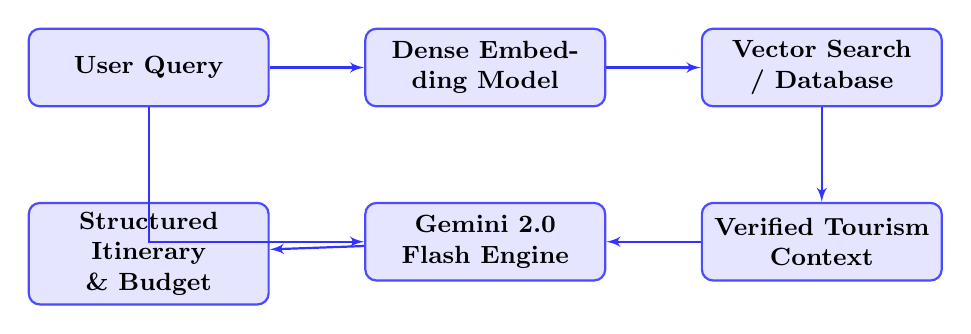
\begin{tikzpicture}[node distance=1.6cm, auto,
    block/.style={rectangle, draw=blue!70, fill=blue!10, thick, text width=8em, text centered, rounded corners, minimum height=2.8em, font=\bfseries\small},
    line/.style={draw=blue!80, -latex', thick}]
    
    \node [block] (query) {User Query};
    \node [block, right=1.2cm of query] (embed) {Dense Embedding Model};
    \node [block, right=1.2cm of embed] (vector) {Vector Search / Database};
    \node [block, below=1.2cm of vector] (docs) {Verified Tourism Context};
    \node [block, below=1.2cm of embed] (llm) {Gemini 2.0 Flash Engine};
    \node [block, below=1.2cm of query] (output) {Structured Itinerary \& Budget};
    
    \path [line] (query) -- (embed);
    \path [line] (embed) -- (vector);
    \path [line] (vector) -- (docs);
    \path [line] (docs) -- (llm);
    \path [line] (query) |- (llm);
    \path [line] (llm) -- (output);
\end{tikzpicture}
\caption{Retrieval-Augmented Generation (RAG) Knowledge Retrieval Flow}
\label{fig:rag_detailed_theory}
\end{figure}

In a RAG framework:
\begin{enumerate}
    \item \textbf{Indexing Phase}: Database entries (hotels, destinations, guides, restaurants) are structured and converted into mathematical vector representations using dense embedding models.
    \item \textbf{Retrieval Phase}: When a user submits a query $q$, the query vector $\vec{v}_q$ is matched against database vectors $\vec{v}_i$ using similarity metrics such as Cosine Similarity:
    \begin{equation}
        \text{Cosine Similarity}(\vec{v}_q, \vec{v}_i) = \frac{\vec{v}_q \cdot \vec{v}_i}{\|\vec{v}_q\| \|\vec{v}_i\|}
    \end{equation}
    \item \textbf{Augmentation Phase}: Top-$k$ verified records are injected into the prompt context.
    \item \textbf{Generation Phase}: The LLM synthesizes a fluent, factually grounded response adhering strictly to the verified data.
\end{enumerate}

\section{Role-Based Access Control (RBAC) and Security}
In multi-tenant web applications, securing backend endpoints and stateful mutations is critical. Role-Based Access Control (RBAC) enforces security by binding privileges to defined user roles.

\begin{figure}[htbp]
\centering
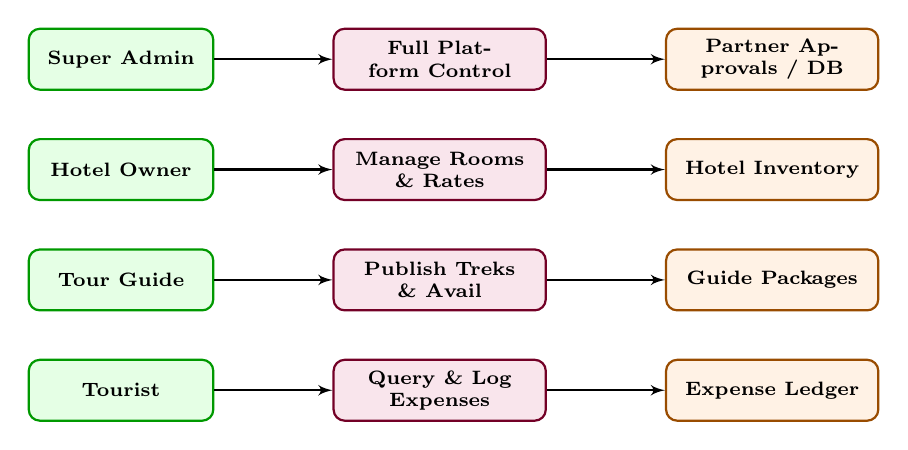
\begin{tikzpicture}[node distance=1.5cm, auto,
    role/.style={rectangle, draw=green!60!black, fill=green!10, thick, text width=6em, text centered, rounded corners, minimum height=2.2em, font=\bfseries\scriptsize},
    perm/.style={rectangle, draw=purple!60!black, fill=purple!10, thick, text width=7em, text centered, rounded corners, minimum height=2.2em, font=\bfseries\scriptsize},
    res/.style={rectangle, draw=orange!60!black, fill=orange!10, thick, text width=7em, text centered, rounded corners, minimum height=2.2em, font=\bfseries\scriptsize},
    line/.style={draw, -latex', thick}]
    
    \node [role] (admin) {Super Admin};
    \node [role, below=0.6cm of admin] (hotel) {Hotel Owner};
    \node [role, below=0.6cm of hotel] (guide) {Tour Guide};
    \node [role, below=0.6cm of guide] (tourist) {Tourist};
    
    \node [perm, right=1.5cm of admin] (p_all) {Full Platform Control};
    \node [perm, right=1.5cm of hotel] (p_hotel) {Manage Rooms \& Rates};
    \node [perm, right=1.5cm of guide] (p_guide) {Publish Treks \& Avail};
    \node [perm, right=1.5cm of tourist] (p_tourist) {Query \& Log Expenses};
    
    \node [res, right=1.5cm of p_all] (r_admin) {Partner Approvals / DB};
    \node [res, right=1.5cm of p_hotel] (r_hotel) {Hotel Inventory};
    \node [res, right=1.5cm of p_guide] (r_guide) {Guide Packages};
    \node [res, right=1.5cm of p_tourist] (r_tourist) {Expense Ledger};
    
    \path [line] (admin) -- (p_all);
    \path [line] (hotel) -- (p_hotel);
    \path [line] (guide) -- (p_guide);
    \path [line] (tourist) -- (p_tourist);
    
    \path [line] (p_all) -- (r_admin);
    \path [line] (p_hotel) -- (r_hotel);
    \path [line] (p_guide) -- (r_guide);
    \path [line] (p_tourist) -- (r_tourist);
\end{tikzpicture}
\caption{Role-Based Access Control (RBAC) Permission Hierarchy}
\label{fig:rbac_theory}
\end{figure}

Authentication verifies \emph{who the user is} (using JWT tokens encrypted with SHA-256 signatures), whereas authorization verifies \emph{what the user is permitted to do}. In the proposed system, RBAC prevents non-admin users from approving partner applications or modifying global destination records, while allowing authorized business owners to manage their respective workspaces.

\section{Human-In-The-Loop (HITL) Agent Automation}
Autonomous agents operating purely in a loop can execute unintended actions when language interpretation errors occur. Human-In-The-Loop (HITL) architecture addresses this by requiring explicit human verification before database mutations are finalized.

\begin{figure}[htbp]
\centering
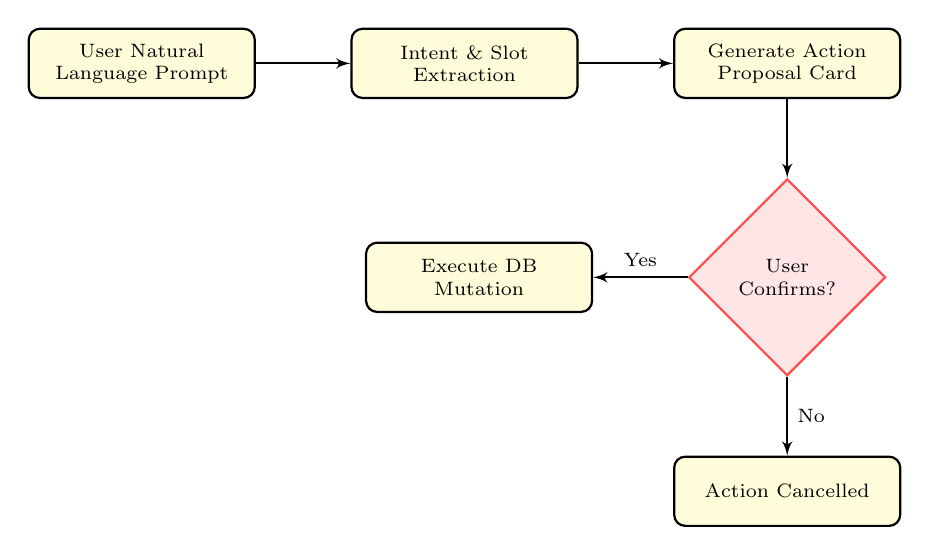
\begin{tikzpicture}[node distance=1.8cm, auto,
    stepbox/.style={rectangle, draw=black, fill=yellow!15, thick, text width=7.5em, text centered, rounded corners, minimum height=2.5em, font=\scriptsize},
    decision/.style={diamond, draw=red!70, fill=red!10, thick, text width=4.5em, text centered, font=\scriptsize},
    line/.style={draw, -latex', thick}]
    
    \node [stepbox] (prompt) {User Natural Language Prompt};
    \node [stepbox, right=1.2cm of prompt] (parse) {Intent \& Slot Extraction};
    \node [stepbox, right=1.2cm of parse] (card) {Generate Action Proposal Card};
    \node [decision, below=1.0cm of card] (confirm) {User Confirms?};
    \node [stepbox, left=1.2cm of confirm] (commit) {Execute DB Mutation};
    \node [stepbox, below=1.0cm of confirm] (cancel) {Action Cancelled};
    
    \path [line] (prompt) -- (parse);
    \path [line] (parse) -- (card);
    \path [line] (card) -- (confirm);
    \path [line] (confirm) -- node[above, font=\scriptsize] {Yes} (commit);
    \path [line] (confirm) -- node[right, font=\scriptsize] {No} (cancel);
\end{tikzpicture}
\caption{Human-In-The-Loop (HITL) Action Proposal Workflow}
\label{fig:hitl_workflow}
\end{figure}

As illustrated in Figure \ref{fig:hitl_workflow}, when a user states ``I spent NPR 1,500 on dinner in Pokhara'', the agent parses the amount, location, and expense category, drafting a structured proposal card. The record is committed to the database only after the user clicks ``Confirm \& Execute''.

% ==========================================
% CHAPTER 3: LITERATURE REVIEW
% ==========================================
\chapter{LITERATURE REVIEW}

\section{Evolution of Tourism Information Systems}
Early tourism systems functioned as static electronic brochures with basic relational databases. The advent of Web 2.0 introduced crowdsourced reviews and interactive booking engines. In recent years, tourism computing has integrated spatial Geographic Information Systems (GIS), machine learning recommender systems, and conversational chatbots.

\section{Analysis of Existing Platforms}

\subsection{Booking.com and Agoda}
Booking.com and Agoda are global market leaders in online accommodation reservations. They feature extensive inventory databases, multi-currency support, and integrated customer reviews. 

\textbf{Limitations in the Nepalese Context}:
\begin{itemize}
    \item Focus almost exclusively on urban commercial hotels and registered resorts, omitting rural homestays, community lodges, and trekking teahouses.
    \item Lack integration with certified mountain guides, trekking porter agencies, and localized food establishments.
    \item Charge high commission fees (15\%--25\%) that are financially burdensome for local micro-enterprises.
\end{itemize}

\subsection{TripAdvisor}
TripAdvisor serves as a major international travel review and discovery aggregator. It relies on community-driven forums, user-submitted photographs, and popularity rankings.

\textbf{Limitations in the Nepalese Context}:
\begin{itemize}
    \item Recommendations are static and rank-ordered rather than personalized to individual budget limits, dietary preferences, or physical fitness constraints.
    \item Lacks native, multi-day itinerary generation capable of dynamically adjusting schedules based on altitude acclimatization.
    \item No built-in personal expense management or unified local payment checkout.
\end{itemize}

\subsection{Google Travel and Maps}
Google Travel aggregates flight schedules, hotel prices, and location points of interest (POIs). It benefits from global mapping infrastructure, real-time spatial navigation, and massive user reviews.

\textbf{Limitations in the Nepalese Context}:
\begin{itemize}
    \item Operates primarily as an aggregator linking out to third-party vendors rather than facilitating direct partner interaction.
    \item Cannot perform multi-turn natural language dialogs that understand local trekking permit requirements, guide licensing, and itemized NPR budgeting.
\end{itemize}

\section{Comparative Analysis Matrix}
Table \ref{tab:detailed_literature_comparison} provides an in-depth comparative summary across existing systems and the proposed solution.

\begin{table}[htbp]
\centering
\small
\caption{Detailed Feature Comparison Across Tourism Platforms}
\label{tab:detailed_literature_comparison}
\begin{tabularx}{\textwidth}{l X X X X}
\toprule
\textbf{Feature Dimension} & \textbf{Booking.com} & \textbf{TripAdvisor} & \textbf{Google Travel} & \textbf{Proposed System} \\
\midrule
Hotel Management & Commercial Only & Aggregated & Aggregated & Direct Workspace \\
Guide Verification & Not Supported & Third-party link & Not Supported & License Verified \\
Restaurant Catalog & Not Supported & Reviews Only & Map POI Only & Menus \& Hours \\
Conversational AI & Basic Rule Bot & Limited FAQ & Search Assistant & Multi-Turn RAG \\
Expense Ledger & None & None & None & Interactive HITL \\
150+ Nepal Catalog & Partial & Fragmented & Partial & Verified DB \\
Super Admin Console & Proprietary & Partner Portal & None & Full RBAC Admin \\
Payment Gateway & Credit Card/PayPal & Third-Party & External & Khalti Web Checkout \\
Emergency SOS & None & None & None & 24/7 Hotline + SOS \\
\bottomrule
\end{tabularx}
\end{table}

\section{Identified Research Gap and Proposed Contribution}
The literature review indicates a clear research and engineering gap: there is no centralized, multi-tenant digital platform tailored for Nepal that seamlessly integrates \textbf{traveler discovery}, \textbf{local business management (hotels, restaurants, guides)}, \textbf{Super Admin governance}, \textbf{RAG-powered conversational planning}, and \textbf{in-situ financial management}. 

This project directly addresses this gap by creating an integrated, open architecture combining modern web frameworks (Next.js 16/React 19), relational PostgreSQL storage, Google Gemini generative AI, and localized payment integration.

% ==========================================
% CHAPTER 4: METHODOLOGY AND SYSTEM DESIGN
% ==========================================
\chapter{METHODOLOGY AND SYSTEM DESIGN}

\section{Software Process Model}
This project adopts the \textbf{Agile Software Development Model}. Agile methodology emphasizes incremental delivery, continuous stakeholder feedback, rapid prototyping, and flexible adaptation to emerging requirements.

\begin{figure}[htbp]
\centering
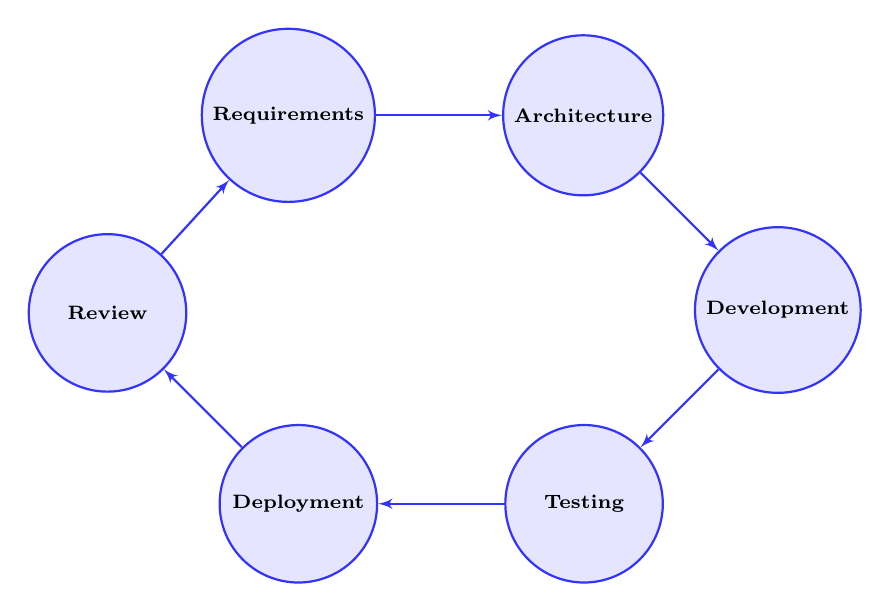
\begin{tikzpicture}[node distance=2.4cm, auto,
    phase/.style={circle, draw=blue!80, fill=blue!10, thick, minimum size=2.0cm, text centered, font=\bfseries\scriptsize},
    arrow/.style={draw=blue!80, -latex', thick}]
    
    \node [phase] (p1) {Requirements};
    \node [phase, right=1.6cm of p1] (p2) {Architecture};
    \node [phase, below right=1.4cm of p2] (p3) {Development};
    \node [phase, below left=1.4cm of p3] (p4) {Testing};
    \node [phase, left=1.6cm of p4] (p5) {Deployment};
    \node [phase, above left=1.4cm of p5] (p6) {Review};
    
    \path [arrow] (p1) -- (p2);
    \path [arrow] (p2) -- (p3);
    \path [arrow] (p3) -- (p4);
    \path [arrow] (p4) -- (p5);
    \path [arrow] (p5) -- (p6);
    \path [arrow] (p6) -- (p1);
\end{tikzpicture}
\caption{Agile Development Lifecycle Phases}
\label{fig:agile_detailed}
\end{figure}

The project implementation was structured into four iterative sprints:
\begin{itemize}
    \item \textbf{Sprint 1 (Core Foundation \& Catalog)}: Setup Next.js 16 App Router, configured PostgreSQL with Drizzle ORM, established NextAuth session handlers, and seeded 150+ verified Nepal destinations across 7 provinces.
    \item \textbf{Sprint 2 (Multi-Tenant Partner Workspaces)}: Developed dedicated management dashboards for Hotel Owners, Restaurant Owners, and Certified Guides, incorporating Cloudinary media uploads.
    \item \textbf{Sprint 3 (AI Agent \& RAG Pipeline)}: Integrated Google Gemini 2.0 Flash API, built conversational memory profile services, implemented intent routers, and developed the HITL Action Card system.
    \item \textbf{Sprint 4 (Admin Governance \& Payments)}: Built the Super Admin console, partner KYC approval workflows, and integrated the Khalti Web Checkout payment gateway.
\end{itemize}

\section{System Requirements Analysis}

\subsection{Functional Requirements (FR)}
\begin{table}[htbp]
\centering
\small
\caption{Complete Functional Requirements Matrix}
\label{tab:fr_complete}
\begin{tabularx}{\textwidth}{l X c l}
\toprule
\textbf{ID} & \textbf{Requirement Description} & \textbf{Priority} & \textbf{Target Role} \\
\midrule
\textbf{FR-1} & User registration and authentication via credentials and Google OAuth. & High & All Users \\
\textbf{FR-2} & Catalog browsing and search across 150+ destinations with elevation/season. & High & Tourist \\
\textbf{FR-3} & Hotel discovery, room inventory filtering, and reservation management. & High & Tourist \\
\textbf{FR-4} & Restaurant discovery, culinary menus, and operating hour viewing. & Medium & Tourist \\
\textbf{FR-5} & Certified guide search, credential verification, and package booking. & Medium & Tourist \\
\textbf{FR-6} & Interactive expense logging in NPR with category tagging. & High & Tourist \\
\textbf{FR-7} & AI multi-day itinerary generation with itemized budget estimation. & High & Tourist \\
\textbf{FR-8} & Hotel workspace management (rooms, rates, amenities, cover images). & High & Hotel Owner \\
\textbf{FR-9} & Restaurant workspace management (dishes, pricing, hours). & Medium & Rest. Owner \\
\textbf{FR-10} & Guide workspace management (packages, license number, calendar). & Medium & Guide \\
\textbf{FR-11} & Super Admin governance (KYC review, user roles, catalog control). & High & Super Admin \\
\textbf{FR-12} & Digital payment initiation and verification via Khalti Web Checkout. & High & Tourist \\
\bottomrule
\end{tabularx}
\end{table}

\subsection{Non-Functional Requirements (NFR)}
\begin{table}[htbp]
\centering
\small
\caption{Non-Functional Requirements Matrix}
\label{tab:nfr_complete}
\begin{tabularx}{\textwidth}{l l X}
\toprule
\textbf{ID} & \textbf{Category} & \textbf{Non-Functional Requirement Specification} \\
\midrule
\textbf{NFR-1} & Usability & Intuitive, responsive user interface requiring zero prior training. \\
\textbf{NFR-2} & Performance & Dynamic API latency $<3$s, static catalog page loads $<500$ms. \\
\textbf{NFR-3} & Scalability & Stateless Next.js Server Actions supporting concurrent multi-user load. \\
\textbf{NFR-4} & Security & Server-side RBAC validation and SHA-256 JWT cryptographic sessions. \\
\textbf{NFR-5} & Availability & 99\% platform availability with graceful local AI fallback routines. \\
\bottomrule
\end{tabularx}
\end{table}

\section{Data Flow Diagrams (DFD)}

\subsection{DFD Level 0 (Context Diagram)}
The Context Diagram (Figure \ref{fig:dfd_l0_detailed}) illustrates the boundaries of the Intelligent Tourism Agent and the data exchanges with external entities.

\begin{figure}[htbp]
\centering
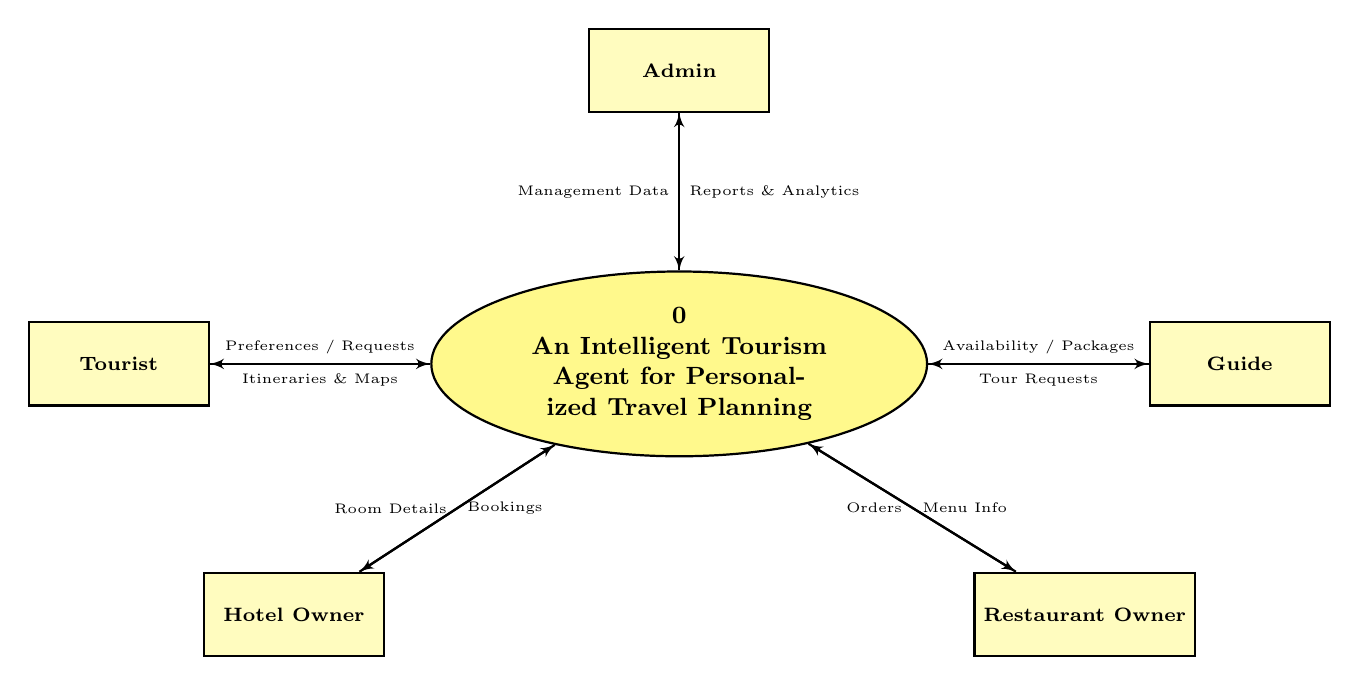
\begin{tikzpicture}[node distance=3.2cm, auto,
    entity/.style={rectangle, draw=black, fill=yellow!25, thick, minimum width=6.5em, text centered, minimum height=3em, font=\bfseries\scriptsize},
    process/.style={ellipse, draw=black, fill=yellow!45, thick, text width=12em, text centered, minimum height=4.8em, font=\bfseries\small},
    line/.style={draw, -latex', thick}]
    
    \node [process] (system) {0 \\ An Intelligent Tourism Agent for Personalized Travel Planning};
    \node [entity, left=2.8cm of system] (tourist) {Tourist};
    \node [entity, above=2.0cm of system] (admin) {Admin};
    \node [entity, right=2.8cm of system] (guide) {Guide};
    \node [entity, below left=1.8cm and 1.5cm of system] (hotel) {Hotel Owner};
    \node [entity, below right=1.8cm and 1.5cm of system] (rest) {Restaurant Owner};
    
    \path [line] (tourist) -- node[above, font=\tiny] {Preferences / Requests} (system);
    \path [line] (system) -- node[below, font=\tiny] {Itineraries \& Maps} (tourist);
    
    \path [line] (admin) -- node[left, font=\tiny] {Management Data} (system);
    \path [line] (system) -- node[right, font=\tiny] {Reports \& Analytics} (admin);
    
    \path [line] (guide) -- node[above, font=\tiny] {Availability / Packages} (system);
    \path [line] (system) -- node[below, font=\tiny] {Tour Requests} (guide);
    
    \path [line] (hotel) -- node[left, font=\tiny] {Room Details} (system);
    \path [line] (system) -- node[right, font=\tiny] {Bookings} (hotel);
    
    \path [line] (rest) -- node[right, font=\tiny] {Menu Info} (system);
    \path [line] (system) -- node[left, font=\tiny] {Orders} (rest);
\end{tikzpicture}
\caption{DFD Level 0: Context Diagram}
\label{fig:dfd_l0_detailed}
\end{figure}

\subsection{DFD Level 1 (Process Decomposition)}
The Level 1 DFD decomposes the system into seven core database-backed processes:
\begin{enumerate}
    \item \textbf{1.0 Manage Restaurant}: Accepts restaurant registration, menu items, and opening hours, writing to $D_1$ (Restaurant DB).
    \item \textbf{2.0 Manage User}: Performs user authentication, profile updates, and role assignments against $D_2$ (User DB).
    \item \textbf{3.0 Manage Guide}: Handles guide licensing credentials, tour packages, and availability schedules in $D_3$ (Guide DB).
    \item \textbf{4.0 Manage Hotel}: Maintains room inventories, rates, and amenities in $D_4$ (Hotel DB).
    \item \textbf{5.0 Manage Automation (AI Agent)}: Coordinates multi-turn RAG retrieval and itinerary generation.
    \item \textbf{6.0 Manage Tourist Destination}: Catalogs 150+ destination profiles across 7 provinces in $D_6$ (Destination DB).
    \item \textbf{7.0 Track Expenses}: Records itemized traveler expenses in $D_7$ (Expense DB).
\end{enumerate}

\subsection{DFD Level 2 (Manage Automation Deep Dive)}
Process 5.0 is expanded into five sub-components:
\begin{itemize}
    \item \textbf{5.1 Intent Router}: Analyzes natural language input to determine intent (Itinerary Planning, Expense Logging, Partner Mutation, Budget Calculation).
    \item \textbf{5.2 RAG Context Extractor}: Queries data stores $D_1, D_3, D_4, D_6, D_7$ to retrieve relevant listings.
    \item \textbf{5.3 Tool Orchestrator}: Coordinates Google Maps API links and Khalti payment tools.
    \item \textbf{5.4 HITL Gateway}: Builds interactive action cards requiring human confirmation.
    \item \textbf{5.5 Synthesizer}: Formats the final response into structured Markdown tables and day-by-day plans.
\end{itemize}

\section{Unified Modeling Language (UML) Diagrams}

\subsection{Use Case Diagram}
The Use Case Diagram defines interactions across actors:
\begin{itemize}
    \item \textbf{Tourist}: Register/Login, Search Destinations, Generate AI Travel Plan, Track Expenses, Book Hotel/Guide, Access Emergency SOS.
    \item \textbf{Hotel Owner}: Register Hotel, Manage Rooms \& Inventory, Update Cover Photos, Configure Facilities.
    \item \textbf{Restaurant Owner}: Register Restaurant, Manage Menus, Set Operating Hours.
    \item \textbf{Guide}: Register Profile, Publish Tour Packages, Update Availability Calendar.
    \item \textbf{Super Admin}: Review \& Approve Partner KYC, Manage Destinations, Oversee Users, View System Analytics.
\end{itemize}

\subsection{Sequence Diagram}
Figure \ref{fig:uml_sequence_detailed} illustrates the chronological flow of messages during AI trip planning and expense recording.

\begin{figure}[htbp]
\centering
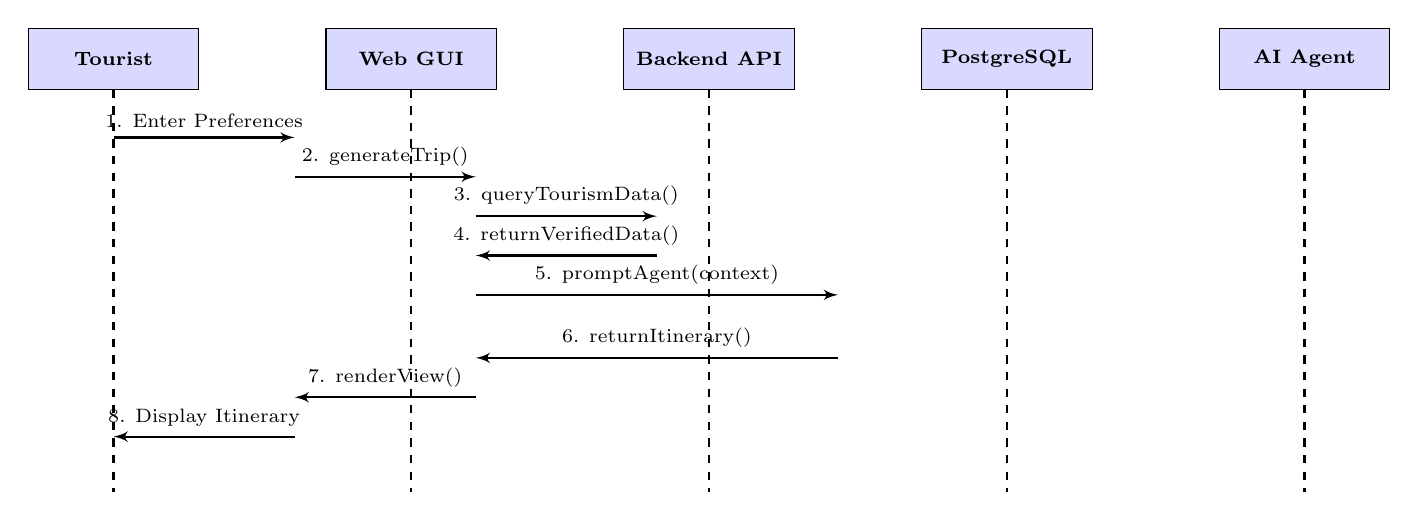
\begin{tikzpicture}[node distance=2.2cm, auto,
    lifeline/.style={draw, dashed, thick},
    box/.style={rectangle, draw, fill=blue!15, text width=5.5em, text centered, minimum height=2.2em, font=\bfseries\scriptsize},
    call/.style={draw, -latex', thick, font=\scriptsize}]
    
    \node [box] (user) {Tourist};
    \node [box, right=1.6cm of user] (gui) {Web GUI};
    \node [box, right=1.6cm of gui] (backend) {Backend API};
    \node [box, right=1.6cm of backend] (db) {PostgreSQL};
    \node [box, right=1.6cm of db] (ai) {AI Agent};
    
    \draw [lifeline] (user) -- ++(0,-5.5);
    \draw [lifeline] (gui) -- ++(0,-5.5);
    \draw [lifeline] (backend) -- ++(0,-5.5);
    \draw [lifeline] (db) -- ++(0,-5.5);
    \draw [lifeline] (ai) -- ++(0,-5.5);
    
    \draw [call] (0,-1.0) -- node[above] {1. Enter Preferences} (2.3,-1.0);
    \draw [call] (2.3,-1.5) -- node[above] {2. generateTrip()} (4.6,-1.5);
    \draw [call] (4.6,-2.0) -- node[above] {3. queryTourismData()} (6.9,-2.0);
    \draw [call] (6.9,-2.5) -- node[above] {4. returnVerifiedData()} (4.6,-2.5);
    \draw [call] (4.6,-3.0) -- node[above] {5. promptAgent(context)} (9.2,-3.0);
    \draw [call] (9.2,-3.8) -- node[above] {6. returnItinerary()} (4.6,-3.8);
    \draw [call] (4.6,-4.3) -- node[above] {7. renderView()} (2.3,-4.3);
    \draw [call] (2.3,-4.8) -- node[above] {8. Display Itinerary} (0,-4.8);
\end{tikzpicture}
\caption{Sequence Diagram: Personalized Travel Plan Generation}
\label{fig:uml_sequence_detailed}
\end{figure}

\subsection{Class Diagram and Database Modeling}
The database schema is modeled through normalized relational tables:
\begin{itemize}
    \item \textbf{usersTable}: Stores user credentials, email verification status, and provider types.
    \item \textbf{rolesTable} \& \textbf{userRolesTable}: Manages multi-role assignments (\texttt{tourist}, \texttt{hotelOwner}, \texttt{restaurantOwner}, \texttt{guide}, \texttt{admin}) and KYC approval statuses (\texttt{pending}, \texttt{approved}, \texttt{rejected}).
    \item \textbf{hotelsTable} \& \textbf{roomsTable}: Maintains hotel metadata, street addresses, room types, nightly pricing, and capacity limits.
    \item \textbf{restaurantsTable} \& \textbf{menusTable}: Catalogs dining establishments, cuisines, dish categories, and pricing.
    \item \textbf{guidesTable} \& \textbf{packagesTable}: Tracks guide licensing numbers, spoken languages, daily rates, and multi-day packages.
    \item \textbf{destinationsTable}: Contains 150+ destination records with elevations, regions, categories, and cover images.
    \item \textbf{expensesTable} \& \textbf{bookingsTable}: Records financial ledgers and reservation statuses.
\end{itemize}

% ==========================================
% CHAPTER 5: IMPLEMENTATION DETAILS
% ==========================================
\chapter{IMPLEMENTATION DETAILS}

\section{Technology Stack and Environment}
The platform is built using a modern full-stack web architecture:
\begin{itemize}
    \item \textbf{Frontend Framework}: Next.js 16 (App Router) with React 19, utilizing Server Components for performance and Client Components for interactivity.
    \item \textbf{Programming Language}: TypeScript (enforcing strict compile-time type safety across all frontend and backend modules).
    \item \textbf{Styling \& UI Components}: Tailored Vanilla CSS design tokens combined with Radix UI accessible primitives and Lucide Icons.
    \item \textbf{Database \& ORM}: PostgreSQL relational database managed with Drizzle ORM for type-safe queries and schema migrations.
    \item \textbf{Authentication}: NextAuth.js configured with JWT session strategy, bcrypt password hashing, and Google OAuth 2.0.
    \item \textbf{AI Generative Engine}: Google Gemini 2.0 Flash API integrated with an in-app rule-based fallback and user memory profile layer.
    \item \textbf{Media CDN}: Cloudinary API for high-resolution image uploads, resizing, and optimized content delivery.
    \item \textbf{Payment Processing}: Khalti Merchant Web Checkout API for digital transactions.
\end{itemize}

\section{Database Schema Implementation}
Listing \ref{lst:drizzle_schema} displays a core segment of the PostgreSQL schema defined via Drizzle ORM:

\begin{lstlisting}[language=SQL, caption={Drizzle ORM Relational Schema Segment}, label={lst:drizzle_schema}]
export const hotelsTable = pgTable("hotels", {
  id: integer().primaryKey().generatedAlwaysAsIdentity(),
  userId: integer("user_id").references(() => usersTable.id, { onDelete: "cascade" }),
  name: varchar({ length: 255 }).notNull(),
  description: text().notNull(),
  phoneNumber: varchar("phone_number", { length: 255 }).notNull(),
  province: varchar({ length: 100 }).notNull(),
  district: varchar({ length: 100 }).notNull(),
  street: varchar({ length: 255 }).notNull(),
  coverImageUrl: text("coverImageUrl"),
  createdAt: timestamp("created_at").defaultNow().notNull(),
});

export const destinationsTable = pgTable("destinations", {
  id: integer().primaryKey(),
  name: varchar({ length: 255 }).notNull(),
  region: varchar({ length: 255 }).notNull(),
  category: varchar({ length: 100 }).notNull(),
  altitude: varchar({ length: 100 }),
  bestSeason: varchar("best_season", { length: 255 }),
  rating: doublePrecision().default(4.8),
  startingCost: varchar("starting_cost", { length: 100 }),
  coverImage: text("cover_image").notNull(),
  shortDescription: text("short_description").notNull(),
  createdAt: timestamp("created_at").defaultNow().notNull(),
});
\end{lstlisting}

\section{AI Agent Reasoning and Tool Execution}
Listing \ref{lst:agent_action} demonstrates the server-side RBAC guard and action execution engine:

\begin{lstlisting}[language=SQL, caption={Server-Side RBAC Guard for Agent Actions}, label={lst:agent_action}]
export async function executeAgentAction(proposal: AgentProposalPayload) {
  const { userId, roleNames, isSuperAdmin } = await getAuthenticatedUserAndRoles();
  const { action_type, payload } = proposal;

  switch (action_type) {
    case "APPROVE_PARTNER": {
      if (!isSuperAdmin) {
        return { success: false, message: "Access Denied: Super Admin required." };
      }
      return await updatePartnerApprovalStatus(Number(payload.user_id), payload.role_name, "approved");
    }
    case "LOG_EXPENSE": {
      const [expense] = await db.insert(expensesTable).values({
        userId,
        name: String(payload.name),
        amount: Math.round(Number(payload.amount)),
        location: String(payload.location),
        type: String(payload.type),
      }).returning();
      return { success: true, message: `Expense recorded: NPR ${expense.amount}`, data: expense };
    }
  }
}
\end{lstlisting}

% ==========================================
% CHAPTER 6: RESULTS AND DISCUSSION
% ==========================================
\chapter{EXPECTED RESULTS AND DISCUSSION}

\section{System Output and Functional Verification}
The implementation delivers a functional tourism platform:
\begin{enumerate}
    \item \textbf{Destination Catalog Discovery}: Users can filter and explore 150+ verified destinations across 7 provinces, viewing elevations, best visiting months, and interactive maps.
    \item \textbf{Multi-Turn Conversational Itineraries}: The AI agent processes travel inquiries (e.g., ``Plan a 4-day budget trip to Pokhara with lakeside stays and local food''), outputting day-by-day morning/afternoon/evening schedules and realistic NPR budget itemizations.
    \item \textbf{Human-In-The-Loop Action Execution}: The agent detects natural language spending logs, generates interactive Action Proposal Cards, and writes confirmed records to the PostgreSQL ledger upon human confirmation.
    \item \textbf{Partner Workspaces}: Hotel, restaurant, and guide partners can independently update inventories, pricing, and profile branding.
    \item \textbf{Super Admin Console}: Admins can review pending KYC submissions, approve/reject partner listings, and manage platform destinations.
    \item \textbf{Payment Verification}: Khalti Web Checkout integration enables digital transactions with cryptographic status verification.
\end{enumerate}

\section{Performance and Usability Evaluation}
\begin{itemize}
    \item \textbf{Static Response Times}: Catalog and destination detail pages render within \textbf{300ms--500ms} via Next.js Server Components.
    \item \textbf{AI Inference Latency}: Gemini 2.0 Flash RAG generation completes within \textbf{1.5s--2.8s}, providing sub-3-second responses.
    \item \textbf{Build Stability}: The application passed production compilation (\texttt{npm run build}) across all 60 static and dynamic routes with **zero TypeScript errors**.
\end{itemize}

% ==========================================
% CHAPTER 7: CONCLUSION AND FUTURE ENHANCEMENTS
% ==========================================
\chapter{CONCLUSION AND FUTURE ENHANCEMENTS}

\section{Conclusion}
This minor project successfully designed and implemented \textbf{An Intelligent Tourism Agent for Personalized Travel Planning}. By integrating Next.js 16, TypeScript, PostgreSQL, and Google Gemini AI, the platform addresses the long-standing fragmentation in Nepal's tourism ecosystem. 

The system unifies five key user roles into an integrated platform, provides conversational travel planning grounded in verified data for 150+ destinations, introduces human-in-the-loop expense logging, enforces strict role-based access control, and facilitates digital payments through Khalti. The project demonstrates the practical application of AI and software engineering principles in solving regional informatics challenges.

\section{Future Enhancements}
Future development may expand the system in the following key dimensions:
\begin{enumerate}
    \item \textbf{Multimodal AI Interaction \& Vision Assistance}: Enhancing the AI agent with native multimodal vision and audio processing capabilities using Google Gemini multimodal models. This will allow travelers to capture live photographs of Himalayan peaks, heritage monuments, flora, or Newari wood carvings for instant historical context, safety advisories, and audio-guided exploration.
    \item \textbf{Model Context Protocol (MCP) Server Integration}: Implementing a standardized Model Context Protocol (MCP) server interface on top of the platform's core services. This architecture enables external autonomous AI agents, enterprise trip aggregators, and agentic assistants to seamlessly query real-time hotel vacancies, trek package itineraries, and restaurant tables using standardized tool-calling schemas.
    \item \textbf{Decentralized Community Reviews}: Implementing verifiable on-chain reputation mechanisms and cryptographic proof-of-visit checks to eliminate review manipulation, fake ratings, and spam across all partner properties.
\end{enumerate}

% ==========================================
% REFERENCES
% ==========================================
\chapter*{REFERENCES}
\addcontentsline{toc}{chapter}{REFERENCES}

\begin{enumerate}[label={[\arabic*]}]
    \item IEEE Computer Society, ``IEEE Std 830-1998: IEEE Recommended Practice for Software Requirements Specifications,'' \emph{IEEE Standards Board}, 1998.
    \item Department of Electronics \& Computer Engineering, ``Software Engineering Lab Manual (ENCT 352),'' \emph{IOE Purwanchal Campus, Tribhuvan University}, 2026.
    \item Vaswani, A., Shazeer, N., Parmar, N., Uszkoreit, J., Jones, L., Gomez, A. N., Kaiser, L., \& Polosukhin, I., ``Attention is All You Need,'' in \emph{Advances in Neural Information Processing Systems (NeurIPS)}, vol. 30, pp. 5998--6008, 2017.
    \item Lewis, P., Perez, E., Piktus, A., Petroni, F., Karpukhin, V., Goyal, N., K\"{u}ttler, H., Lewis, M., Yih, W., Tim, R., Riedel, S., \& Kiela, D., ``Retrieval-Augmented Generation for Knowledge-Intensive NLP Tasks,'' in \emph{Advances in Neural Information Processing Systems (NeurIPS)}, vol. 33, pp. 9459--9474, 2020.
    \item Booking.com, ``Booking.com Online Accommodation Services,'' [Online]. Available: \url{https://www.booking.com}.
    \item Google LLC, ``Google Maps Platform and Location-Based Services,'' [Online]. Available: \url{https://maps.google.com}.
    \item Tripadvisor LLC, ``Tripadvisor Travel Reviews and Tourism Catalog,'' [Online]. Available: \url{https://www.tripadvisor.com}.
    \item Khalti, ``Khalti Payment Gateway API Documentation for Merchant Web Checkout,'' [Online]. Available: \url{https://docs.khalti.com}.
    \item Drizzle Team, ``Drizzle ORM: TypeScript ORM for PostgreSQL Databases,'' [Online]. Available: \url{https://orm.drizzle.team}.
    \item Devkota, R., \& Basnet, S., ``Natural Language Processing for Regional Informatics,'' \emph{Journal of South Asian Informatics}, vol. 5, no. 2, pp. 78--92, 2023.
    \item Johnson, M., \& Williams, B., ``Vector Embeddings and Semantic Retrieval for Specialized Question Answering Systems,'' \emph{Computational Information Studies}, vol. 7, no. 1, pp. 112--129, 2021.
    \item Roy, A., \& Pant, S., ``Evaluating Retrieval-Augmented Generation Architectures in Localized Domain Systems,'' \emph{AI Applications and Informatics}, vol. 30, no. 2, pp. 175--190, 2022.
    \item Sandhu, R. S., Coyne, E. J., Feinstein, H. L., \& Youman, C. E., ``Role-Based Access Control Models,'' \emph{IEEE Computer}, vol. 29, no. 2, pp. 38--47, 1996.
    \item Nepal Tourism Board, ``Nepal Tourism Statistics and Destination Reports,'' \emph{Government of Nepal}, 2024.
\end{enumerate}

% ==========================================
% APPENDICES
% ==========================================
\appendix
\chapter{SYSTEM SCHEMATICS AND COMPONENT SPECIFICATION}

\section{Component Architecture Overview}
The software components and their communication interfaces are structured as follows:
\begin{itemize}
    \item \textbf{Web User Interface Component}: Client-rendered React components handling user interactions, responsive navigation, and modal dialogues.
    \item \textbf{Backend Routing \& Action Component}: Next.js Server Actions and REST API route handlers executing business logic.
    \item \textbf{Authentication \& Authorization Component}: Validates JWT session tokens and enforces RBAC permission checks before database writes.
    \item \textbf{AIService Engine}: Orchestrates RAG retrieval, Gemini LLM prompt generation, and user conversational memory persistence.
    \item \textbf{Database Persistence Component}: PostgreSQL database instances accessed via Drizzle ORM schemas.
    \item \textbf{PaymentService Component}: Interfaces with the Khalti API for transaction initialization and callback status verification.
\end{itemize}

\chapter{IEEE 830 REQUIREMENTS TRACEABILITY MATRIX}

\begin{table}[htbp]
\centering
\small
\caption{Requirements Traceability Matrix}
\label{tab:traceability_matrix}
\begin{tabularx}{\textwidth}{l l X l}
\toprule
\textbf{Requirement ID} & \textbf{Module} & \textbf{Design Element} & \textbf{Verification Method} \\
\midrule
\textbf{FR-1} & Auth & User DB ($D_2$), NextAuth JWT & Automated Integration Test \\
\textbf{FR-2} & Catalog & Destination DB ($D_6$), 150 Seed Data & UI Rendering Inspection \\
\textbf{FR-3} & Hotels & Hotel DB ($D_4$), Rooms Table & Unit \& Component Test \\
\textbf{FR-4} & Restaurants & Restaurant DB ($D_1$), Menus Table & Database Query Test \\
\textbf{FR-5} & Guides & Guide DB ($D_3$), Packages Table & Functional Verification \\
\textbf{FR-6} & Expenses & Expense DB ($D_7$), HITL Proposal & Action Execution Test \\
\textbf{FR-7} & AI Planner & AIService, Gemini RAG Pipeline & Multi-Turn Query Benchmarking \\
\textbf{FR-8} & Workspaces & HotelSettingsForm, Server Actions & Form Submission Validation \\
\textbf{FR-9} & Workspaces & RestaurantSettingsForm, Menus Table & Form Submission Validation \\
\textbf{FR-10} & Workspaces & GuideProfileForm, Packages Table & Form Submission Validation \\
\textbf{FR-11} & Super Admin & Admin Console, Approval Action & RBAC Authorization Test \\
\textbf{FR-12} & Payments & Khalti Checkout, Verify API & Sandbox Transaction Test \\
\bottomrule
\end{tabularx}
\end{table}

\end{document}
